\documentclass[fleqn,14pt]{article}

\usepackage{amsmath}
\usepackage{graphicx}
\usepackage{latexsym}
\usepackage[spanish]{babel}
\usepackage[utf8]{inputenc}
\usepackage{amssymb, amsmath, amsbsy} % simbolitos
\usepackage{enumerate}
\usepackage{anysize}
\usepackage{multirow, array} % para las tablas
\usepackage{booktabs}
\usepackage{color}
\usepackage{wrapfig}
\graphicspath{ {images/} }

%PREÁMBULO
\title{Ejercicios Proceamiento Digital Avanzado en Comunicaciones}
\author{Javier Fern\'andez Morata}
\marginsize{1cm}{1cm}{1cm}{2cm}

%DOCUMENTO
\begin{document}
\maketitle
\pagenumbering{arabic}

%Primer Ejercicio
\section*{Cuesti\'on 5 \-- Junio 17/18 }
\paragraph{Enunciado}
Considere un sistema OFDM que opera a una frecuencia de 3GHz, con un tiempo de símbolo $Ts = 4\cdot10^{-8} s$, $N = 1.760$ portadoras totales(de las cuales se reservan 80 portadoras de guarda en cada uno de los extremos) y un prefijo cíclico de longitud NPC = 100. En este sistema se insertan pilotos cada 10 portadoras y cada 10 símbolos. El sistema tiene un transmisor fijo y un receptor móvil, emplea modulación 8PSK y codificación de canal 1/3. Se pide:
\begin{enumerate}[a)]
  \item Calcular el tiempo de dispersión máximo para que el sistema funcione correctamente. [0.7 puntos]
  \item Calcular la velocidad máxima para que se estime de forma efectiva el canal. [0.5 puntos]
  \item Calcular la tasa neta de transmisión. [0.6 puntos]


  Suponga ahora que en el sistema se definen \textit{resource blocks} de 10 portadoras y 10 símbolos (de forma que sólo se tiene un piloto en cada \textit{resource block}) y que el transmisor sirve a dos usuarios cuyas SNRs instantáneas normalizadas se distribuyen (para cada una de las portadoras) de acuerdo a lo indicado en la siguiente tabla:
  \newline
  \newline
    \begin{table}[ht]
      \centering
      \begin{tabular}{@{}|c|l|l|l|@{}}
      \toprule
      \multicolumn{2}{|c|}{\textbf{CANAL USUARIO 1}} & \multicolumn{2}{l|}{\textbf{CANAL USUARIO 2}} \\ \midrule
      $\gamma$ & \textit{Probabilidad} & $\gamma$   & \textit{Probabilidad}         \\ \midrule
      3        & $\frac{1}{5}$           & 6          & $\frac{3}{5}$               \\ \midrule
      5        & $\frac{2}{5}$           & 7          & $\frac{1}{5}$               \\ \midrule
      12       & $\frac{2}{5}$           & 10         & $\frac{1}{5}$               \\ \midrule
      \end{tabular}
    \end{table}

  \item Calcule la tasa neta media de transmisión para cada uno de los usuarios en los siguientes casos: [0.6 puntos]
  \begin{enumerate}[1.]
    \item Si se realiza un acceso fijo en el que cada uno de los resource blocks se asigna de forma alterna a un usuario.
    \item Si se realiza un acceso oportunista.
  \end{enumerate}
\end{enumerate}

\paragraph{Solución}
\begin{enumerate}[a)]
  %Primer apartado
  \item Para hallar el tiempo de dispersión máximo del sistema, nos ayudaremos tanto de la inserción de pilotos, como de las muestras usadas para el prefijo cíclico, eligiendo así el tiempo de dispersión máximo más restrictivo, asegurandonos así de que el sistema funcione.

  $\bullet$ \textbf{Prefijo Cíclico}: Como ya sabemos, las muestras del prefijo cíclico se escogen de manera que:
  \newline

  \centering {${N_{PC} \cdot Ts>\tau_{max}} \rightarrow  {100 \cdot 4\cdot10^{-8} > \tau_{max}} \rightarrow {\boxed{\tau_{max} = 4\mu s}}$}

  \raggedright
  $\bullet$ \textbf{Pilotos Portadoras}: Tal y como nos dicen en el enunciado, se insertan pilotos, donde el periódo de esta inserción de pilotos es de 10 (1 piloto cada 10 portadoras, y 10 símbolos OFDM).

  Por tanto, la periodicidad de la inserción de pilotos en las portadoras viene dada por el ancho de banda de coherencia, donde:


\centering
$N_t \cdot B_N < B_{ch}$, donde $B_N$ es el ancho de banda de cada subportadora $ \rightarrow B_N = \frac{B}{N} = \frac{1}{T_s \cdot N} = 14'20 kHz$

$N_f \cdot B_N < B_{ch} \rightarrow B_{ch} > 142 kHz \rightarrow \boxed{B_{ch} = 142 kHz}$

\raggedright
El $B_{ch}$ viene determinado por la disperión máxima de manera que $\rightarrow B_{ch} = \frac{1}{3 \cdot \tau_{max}}$. Quedando así que la dispersión máxima: $\boxed{\tau_{max} = 2'34 \mu s}$

Por tanto, para que el sistema funcione correctamente, elegimos el retardo más restrictivo que en este caso es:
\begin{center}
  $\boxed{\tau_{max} = 4\mu s}$
\end{center}
%Segundo Apartado
  \item Para el cálculo de la velocidad necesitamos hallar el tiempo de coherencia del canal ($T_{ch}$), que determina el tiempo en el que el canal se mantiene constante y que viene dado por:
  \begin{center}
    $T_{ch}=\frac{1}{3 \cdot fd_{max}}$, donde $fd_{max}$ es la disperión máxima en frecuencia, donde esta depende de la velocidad del móvil $fd_{max} = \frac{v}{c} \cdot fc$
  \end{center}

  En este sistema, insertamos pilotos cada 10 símbolos OFDM, de manera que $N_t \cdot T_{sOFDM} < T_{ch}$ donde

  $T_{sOFDM} = (N + N_{PC}) \cdot T_s = (1760 + 100) \cdot 4 \cdot 10^{-8} = 74'4 \mu s \rightarrow \boxed{T_{sOFDM} = 74'4 \mu s}$

  $N_t \cdot 74'4 \mu s < T_{ch} \rightarrow \boxed{T_{ch} = 0'744 ms}$

  Tal y como hemos demostrado antes: $fd_{max} = \frac{1}{3 \cdot T_{ch}} = \frac{1}{3 \cdot 0'744 ms} = \boxed{448'02 Hz = fd_{max}}$

  Por tanto, la velocidad maxima del sistema es:

  \centering
  $fd_{max} = \frac{v}{c}\cdot fc \rightarrow v = fd_{max} \cdot \frac{c}{fc} = 448'02 \cdot \frac{3\cdot10^{8}}{3\cdot10^{9}} = \boxed{44'8 m/s = v }$

  \raggedright

  \item Para el cálculo de la tasa de transmisión, hay que tener en cuenta la pérdida por la inserción de pilotos.

\centering

$L_P = \frac{1}{Nt} \cdot \frac{1}{Nf} = \frac{1}{10} \cdot \frac{1}{10} = 0'01 $

\raggedright
Mientras que las pérdidas por prefijo cíclico son:
\begin{center}
  $L_{PC} = 1 - \frac{N}{N+N_{PC}} = 1 - \frac{1760}{1760+100} = 0'05$
\end{center}

Por tanto la tasa neta es:
\begin{center}
    $ R = \frac{k}{T_{sOFDM}} \cdot (1-L_P) \cdot (1-L_{PC}) \cdot r \cdot N = \frac{3}{74'4 \mu s} \cdot 0'99 \cdot 0.95 \cdot \frac{1}{3} \cdot 1760 =  \boxed{22'24 Mbps = R_b}$
\end{center}

\item

  \begin{enumerate}[1.]
    \item Al ser una asignación alterna de bloques la tasa de cada usuario vendrá dada por:
    \begin{center}
      $R_{U1} = R_{U2} = R \cdot P_U$ , donde la probablidad es $\frac{1}{2} \rightarrow R_{U1} = R_{U2} = 22'24 \cdot 10^6 \cdot \frac{1}{2} = \boxed{11'12 Mbps = R_{U1} = R_{U2}} $
    \end{center}
    \item Al realizarse un acceso oportunista, hay que hallar la probablidad de cuando transmite el U1 o el U2. Es decir cuando la SNR del U1 sea mayor que la del U2, transmitira el U1.

    $P_{U1} = P[\gamma_1 > \gamma_2 | \gamma_2] \cdot P[\gamma_2] = 1 - P[\gamma_1 \leq \gamma_2] = 1 - (P[\gamma_1 = 12 | \gamma_2 = 6] \cdot P[\gamma_2 = 6] +   P[\gamma_1 = 12 | \gamma_2 = 7] \cdot   P[\gamma_2 = 7] + P[\gamma_1 = 12 | \gamma_2 = 10] \cdot P[\gamma_2 = 10] ) = 1 - ( \frac{2}{5}\cdot \frac{3}{5} + \frac{2}{5}\cdot \frac{1}{5}  + \frac{2}{5}\cdot \frac{1}{5} = \frac{3}{5} = P_{U1}$
    \newline
    \newline
    Por tanto, la probabilidad de que transmita el Usuario 2 es: $P_{U2} = 1 - P_{U1} = \frac{2}{5}$
    \newline
    Así, las tasas de cada usuario son:
    \begin{center}
      $R_{U1} = R \cdot P_{U1} = 22'4 Mbps \cdot \frac{3}{5} = \boxed{13'44 Mbps = R_{U1}}$\\
      $R_{U2} = R \cdot P_{U2} = 22'4 Mbps \cdot \frac{2}{5} = \boxed{8'96 Mbps = R_{U2}}$
    \end{center}
  \end{enumerate}
\end{enumerate}

\newpage



%Segundo Ejercicio -------------------------------------------------------------------------------------------------------------
\section*{Cuesti\'on 2 \-- Junio 17/18 }
\paragraph{Enunciado}
Considere un sistema de comunicaciones adaptativo y sin ningún tipo de codificación operando sobre un canal móvil con una SNR normalizada que se distribuye como se muestra en la figura inferior (tenga en cuenta que la figura muestra la CDF y no la PFD).


\centering
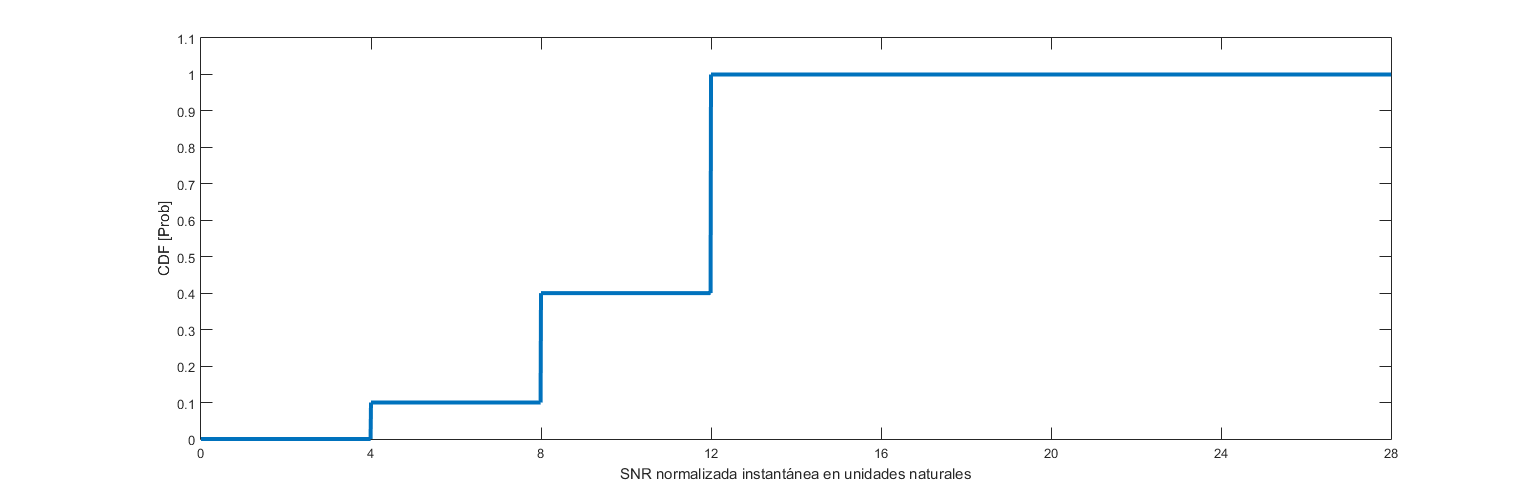
\includegraphics[scale=0.35]{images/imagen}
\raggedright

El sistema opera en un ancho de banda de 1MHz y considera tres modos de transmisión:

\begin{itemize}
  \item Si la SNR instantánea en el receptor es menor que 3dB, no se transmite
  \item Si la SNR instantánea en el receptor es mayor o igual que 3dB y menor que 10dB, se transmite con una potencia de 1W y una modulación 8PSK con un codificador de canal de tasa 1/3 y ganancia de codificación de 4.
  \item Si la SNR instantánea en el receptor es mayor o igual que 10dB, se transmite con una potencia de 2W y una modulación 8PSK sin codificación.
\end{itemize}

Si $\gamma$ denota la SNR instantánea sin codificación y M el tamaño de la constelación, la BER instantánea del sistema puede aproximarse como:

\begin{center}
  $P_e = 0.2 \cdot e^{\frac{-1.5 \gamma}{M-1}}$
\end{center}

\begin{enumerate}[a)]
  \item Calcule cuál es la potencia media de transmisión. Justifique brevemente su repuesta.

  \item Calcule cuál es la BER media en el receptor. Justifique brevemente su repuesta.

  \item Suponga ahora que en el receptor existen 3 antenas y que se implementa un esquema MRC. Calcule la nueva PDF en el receptor y use esa PDF para evaluar la tasa media de transmisión. No hace falta que dibuje la PDF, es suficiente con que calcule la tasa media y justifique el valor.

\end{enumerate}

\paragraph{Soluci\'on}
\begin{enumerate}[a)]
  \item Para poder hallar la potencia media, debemos hallar la probabilidad con la que usamos la potencia, es decir, la probabilidad de cada nodo de tranmsión. Para ello, lo primero es pasar la CDF a PDF. Como sabemos estas vienen relacionadas de tal manera que:

  \begin{center}
    $pdf(x) = \frac{\partial(cdf(x))}{\partial x}$
  \end{center}

  Por tanto, la pdf de nuestra problema es:

  \centering
  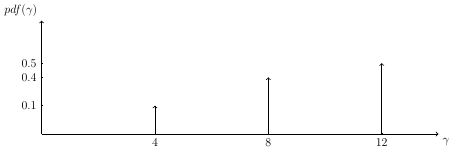
\includegraphics{images/pdfCuestion2_17_18.png}

  \raggedright
  Los intervalos de los modos de transmisión pasados a unidades naturales son:
  \begin{center}
    $\gamma < 2 \rightarrow P_{Tx} = 0 , \  NO \ TX$ \\
    $2 \leq \gamma < 10 \rightarrow P_{Tx} = 1 W, \ 8PSK con\ cod$\\
    $\gamma \geq 10 \rightarrow P_{Tx} = 2 W,\ 8PSK\ sin \ cod$
  \end{center}

  Usando la pdf resultante, podemos hallar las probabilidades de las modulaciones:
  \begin{itemize}
    \item No Tx: $P[NO \ TX] = P[\gamma < 2] = 0$
    \item 8PSK con cod. : $P[8PSK\ con \ cod.] = P[2 \leq \gamma < 10] = P[\gamma = 4] + P[\gamma = 8] = 0.1 + 0.4 = 0.5$
    \item 8PSK sin cod. : $P[8PSK\ sin \ cod.] = P[\gamma \geq 10] = P[\gamma = 12] = 0.5$
  \end{itemize}

  Por tanto, la potencia media de transmisión será:\\
  \begin{center}
    $\overline{P_{Tx}} = 1 W \cdot P_{8PSK-cod} + 2 w \cdot P_{8PSK} = 1 \cdot 0.5 + 2 \cdot 0.5 = \boxed{1.5 W = \overline{P_{Tx}}}$
  \end{center}

  \item Para hallar la $\overline{BER}$, tenemos que hallar las tasas de cada modulación y las probabilidades de error de cada nodo de transmisión.\\
  Es decir:\\
  \centering
  $\overline{BER} = \frac{BER_{8PSK-cod} \cdot Rb_{8PSK-cod} + BER_{8PSK-nocod} \cdot Rb_{8PSK-nocod}}{\overline{Rb}}$

  \raggedright
  \begin{itemize}
    \item   $BER_{8PSK-cod} = (BER(\gamma=4)\cdot 0.1) + (BER(\gamma=8)\cdot 0.4)\ siendo\ BER(\gamma) = 0.2 \cdot exp(\frac{-1.5\cdot \gamma}{M - 1})$. Al tener una modulación con ganancia de codificación tenemos que multiplicar la snr instantánea por dicha ganancia, teniendo para esta modulación la siguiente expresión de $BER(\gamma)$.
    \begin{center}
      $BER(\gamma) = 0.2 \cdot exp(\frac{-1.5 \cdot \gamma \cdot g_c }{M - 1})$
    \end{center}
    \raggedright
    Teniendo así como resultado $\rightarrow$ $\boxed{BER_{8PSK-cod} = 7.32\cdot 10^{-4}}$\\
    \item $BER_{8PSK-nocod} = BER(12) \cdot 0.5 = \boxed{7.64\cdot 10^{-3} = BER_{8PSK-nocod}}$\\
    \item $Rb_{8PSK-cod} = B\cdot k \cdot r$, siendo $ k = log_2 (M) $ y r la tasa de codificación $\rightarrow$ $\boxed{Rb_{8PSK-cod} = 1 Mbps}$\\
    \item $Rb_{8PSK-nocod} = B\cdot k \rightarrow \boxed{Rb_{8PSK-nocod} = 3Mbps}$
    \item $\overline{Rb} = (0.5 \cdot Rb_{8PSK-cod}) + (0.5 \cdot Rb_{8PSK-nocod}) = (0.5 \cdot 1 Mbps) + (0.5 \cdot 3 Mbps) = 2Mbps $
  \end{itemize}

  Así la $\overline{BER}$ del sistema es:\\
  \centering
  $\overline{BER} = \frac{(7.32\cdot 10^{-4} \cdot 1 Mbps) + (7.64\cdot 10^{-3} \cdot 3Mbps)}{2 Mbps} = \boxed{0.01 = \overline{BER}}$\\
  \raggedright
  \item Al implementar en el receptor un esqueme MRC, tenemos que $\gamma_{MRC} = \gamma_1 + \gamma_2 + \gamma_3$ y por consecuencia $pdf(\gamma_{MRC}) = pdf(\gamma_1)*pdf(\gamma_2)*pdf(\gamma_3)$ siendo $\gamma_i$ la snr de la antena i.

  Tras la convolución de las pdfs de los canales, la snr mínima del canal tras el MRC será 12, por lo que la tasa media de transmisión es igual que la tasa transmitida para la modulación de 8PSK sin codificación, ya que dicha modulación se activa cuando la snr es mayor que 10. Por tanto:\\
  \begin{center}
    $\overline{Rb_{sist-MRC}} = Rb_{8PSK-nocod} = B \cdot k = 1 MHz \cdot 3 = \boxed{3 Mbps = \overline{Rb_{sist-MRC}}}$
  \end{center}
\end{enumerate}



%%%%%%%%%%%%%%%%%%%%%%%%%%%%%%%%%%%%%%%%%%%%%%%%%%%%%%%%%%%%%%%%%%%%%%%%%%%%%%%%%%%%%%%%%%%%%%%%%%%%%%%%%%%%%%%%%%%%%%%%
%Ejercicio Revisado 1
\newpage
\section*{Ejercicio 4}
\paragraph{Enunciado}
Considere un sistema $TDMA$ con $8$ usuarios operando sobre un canal Rayleigh de ancho de banda de $10MHz$ con una $SNR$ media de $10dB$ y un tiempo de coherencia de $0.3ms$. El sistema transmite utilizando tramas de longitud $1000$ s\'imbolos. Los primeros $7$ s\'imbolos de cada trama se utilizan para estimar el canal y los $3$ siguientes para identificar el usuario  que accede al mismo. Cada usuario puede transmitir con una potencia media de $1W$.\\
Suponga que el sistema implementa un acceso fijo en el que la primera trama se asigna al usuario $1$, la segunda al usuario $2$ y as\'i sucesivamente hasta el usuario $8$. Una vez que se llega al usuario $8$, la siguiente trama se asigna de nuevo al usuario $1$ y este proceso se repite peri\'odicamente. Suponga adem\'as que los usuarios transmiten con una modulaci\'on $8PSK$ no adaptativa y que, para estas condiciones, la probabilidad de $outage$ es del $10\%$.
\begin{enumerate}[a)]
  \item Indique si cada usuario puede estimar correctamente el canal.
  \item Indique cu\'al es el grado de diversidad para cada usuario.
  \item Indique cu\'al es la tasa de transmisi\'on media neta para cada uno de los usuarios.
  \item Si la trama ha sido asignada a un usuario determinado(por ejemplo, al usuario 1), indique cu\'al es la potencia instant\'anea con la que transmitir\'a el usuario 1 durante esa trama.
  \newline
  \newline
  Suponga ahora que el sistema implementa un acceso adaptativo en el que cada trama se asigna al usuario con mejor $SNR$ instant\'anea. La configuraci\'on del resto del sistema se mantiene igual.
  \item Indique cu\'al es el grado de diversidad para cada usuario.
  \item Indique cu\'al es la tasa de transmisi\'on media neta para cada uno del los usuarios.
\end{enumerate}
\paragraph{Soluci\'on}
\begin{enumerate}[a)]
  \item Para que se pueda estimar bien el canal se tiene que cumplir que:
  $\frac{T_{ch}}{2} > T_{trama} \Rightarrow$ Como tenemos tramas de 1000 s\'imbolos $\Rightarrow T_{trama} = 1000 \cdot T_{s} = 1000 \cdot \frac{1}{B} = \boxed{0.1ms = T_{trama}}$
  Como ya tenemos el $T_{trama}$ podemos comprobar si se estima bien el canal o no:

  \centering
  $\frac{T_{ch}}{2} = \frac{0.3}{2} = 0.15 ms > 0.1 ms \Rightarrow$ Estamos estimando correctamente el canal.

  \raggedright
  \item En el enunciado nos dicen que los usuarios transmiten con una modulaci\'on 8PSK no adaptativa, por tanto por ser un canal Rayleigh y tener una modulac\'on no adaptativa la diversidad es $d=1$.

  \item Para hallar la tasa de cada usuario, hay que tener en cuenta la probabilidad con la que transmite el usuario. Al ser TDMA, y de acceso fijo $\rightarrow P_{TxU} = \frac{1}{N_{US}} = \frac{1}{8}$
  \begin{center}
    $R_{bU} = P_{TxU} \cdot B \cdot log_2(M) \cdot (1 - P_{out}) = \frac{1}{8} \cdot 10MHz \cdot 3 \cdot (1 - 0'1) = \boxed{3'375 Mbps = R_{bU}}$
  \end{center}

  \item Como sabemos la $P_{medU} = 1W$, por tanto la $P_{instU} = \frac{P_{medU}}{P_{TxU}} = \boxed{8 W = P_{instU}}$

  \item La diversidad del canal Rayleigh es 1.

  Como en este caso tenemos una modulaci\'on adaptativa, existir\'a diversidad multiusuario. Tenemos 8 usuarios operando sobre el canal $Rayleigh$, nos quedamos con el mejor de 8 usuarios, y por tanto la diversidad es $d=1 \cdot 8=8$

  \item Calculamos primero $P_{out}^{'}$:
  \begin{center}
    $P_{out}^{'} = (P_{out})^{d} = 0'1^8 = 1 \cdot 10^{-8}$

    $R_{bU} = P_{TxU} \cdot B \cdot log_2(M) \cdot (1 - P_{out}^{'}) = \frac{1}{8} \cdot 10MHz \cdot 3 \cdot (1 - 1 \cdot 10^{-8}) = \boxed{3'75 Mbps = R_{bU}}$
  \end{center}
\end{enumerate}

%%%%%%%%%%%%%%%%%%%%%%%%%%%%%%%%%%%%%%%%%%%%%%%%%%%%%%%%%%%%%%%%%%%%%%%%%%%%%%%%%%%%%%%%%%%%%%%%%%%%%%%%%%%%%%%%%%%%%%%%%%%%%%%%%
%Ejercicio Revisado 2
\newpage
\section*{Ejercicio II.18}
\paragraph{Enunciado}
Para el envío de información entre un transmisor y un recepttor se dispone de dos canales, dichos canales son selectivos en el tiempo pero no siguen una distribución Rayleigh, en concreto, la pdf de la SNR para cada uno de ellos se muestra en la Figura.


  \begin{figure}[htbp]
    \centering
    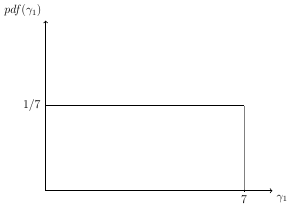
\includegraphics{images/enunciado18(gamma1)}
    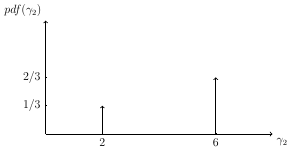
\includegraphics{images/gamma2}
    \caption{pdf de SNR de los canales}
  \end{figure}

Teniendo en cuenta lo anterior:
\begin{enumerate}[1.]
  \item Indique cuál es la pdf de la SNR en el receptor si el transmisor envía la misma información
  por ambos canales y el receptor implementa una técnica de Selection Combining
  (SC). \\
  \item Indique cuál es la pdf de la SNR en el receptor si el transmisor envía la misma información por ambos canales y el receptor implementa una técnica de Maximum Ratio Combining (MRC).
\end{enumerate}

Para los siguientes tres apartados considere que se utiliza únicamente el primero de los canales. Considere además que se utiliza la técnica de transmisión adaptativa que se describe a continuación. El transmisor transmitirá con una potencia fija de 1 W, utilizará un codificador 1/2 y podrá utilizar las tres modulaciones siguientes: BPSQ, QPSK y 8-PSK. El transmisor podrá por tanto encontrarse en cuatro estados (uno para cada modulación más un cuarto estado en el que decide no transmitir). La transición de una modulación a otra se producirá cuando la BER instantánea sea menor que $10^{-2}$

  \begin{enumerate}[1.]
    \item[3.] Calcule cúales son los valres de SNR (conocidos como umbrales) que provocan que el transmisor cambie de una modulación a otra. Para ello calcule previamente la eficiencia espectral para cada uno de los estados y tenga en cuenta que la $BER$ instantánea puede aproximarse como $BER = 0.2exp(-\gamma / (2^R-1))$ donde $\gamma$ denota la SNR instantánea y R es la eficiencia espectral del esquema de modulación-codificación utilizado.
    \item[4.] Calcule la tasa media transmitida por el sistema
    \item[5.] Calcule la BER media del sistema
  \end{enumerate}

Para los siguientes dos apartados considere que se utiliza únicamente el segundo de los canales.

  \begin{enumerate}[1.]
    \item[6.] Calcule cuál es la capacidad media (ergódica) del canal si el transmisor no implementa \textit{waterfilling}
    \item[7.] Calcule cuál es la capacidad media (ergódica) del canal si el transmisor implementa \textit{waterfilling}
  \end{enumerate}

Finalmente, para los dos siguientes apartados considere que el receptor implementa un esquema MRC y que, por tanto, la SNR efectiva es la que ha obtenido en el apartado b).

  \begin{enumerate}[1.]
    \item[8.] Si el transmisor implementa un esquema de transmisión adaptativo de manera que la potencia transmitida es inversamente proporcional a la SNR en el receptor, indique cuál es la potencia media de transmisión y cuál es la SNR que se mediría en el receptor.
    \item[9.] Si el transmisor no implementa ningún esquema de transmisión adaptativo y transmite con potencia y modulación constante, indique cuál es el nivel (ganancia) de diversidad del sistema. Justifique brevemente su respuesta.
  \end{enumerate}

  %Solución
  \paragraph{Soluci\'on}
  \begin{enumerate}[1.]
    \item Como en el receptor se implemento un SC, la pdf del canal resultante sera $\gamma_{SC}=max(\gamma_1,\gamma_2) = pdf_{\gamma_1}(\gamma_1) \cdot pdf_{\gamma_2}(\gamma_2)$. Al tener canales independientes, la pdf conjunta de $\gamma_{SC}$ es la multiplicación de los canales 1 y 2.

    Para mostrar gráficamente los cálculos, vamos a hacerlos mediante la multiplicación de las CDF, cuya relación con la PDF es:
    \begin{center}
      $F(\gamma) = \int_{-\infty}^{\gamma} pdf(\gamma)d\gamma$
    \end{center}

    Por tanto las cdfs de los canales son:


    \begin{displaymath}
      $$cdf(\gamma_1) = \left\{ \begin{array}{ll}
        \frac{\gamma_1}{7} &   0 < \gamma_1 \leq 7 \\
        1 & {\gamma_1 > 7} \\
    \end{array} \right.$$
    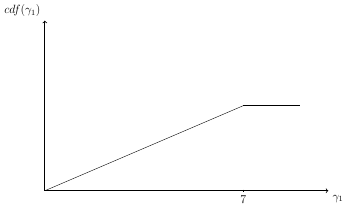
\includegraphics[scale=0.7]{images/cdf1}
    \end{displaymath}


    \begin{displaymath}
      $$cdf(\gamma_2) = \left\{ \begin{array}{ll}
        \frac{1}{3} &   2 < \gamma_2 \leq 6 \\
        1 & \gamma_2 > 6
      \end{array} \right. $$
      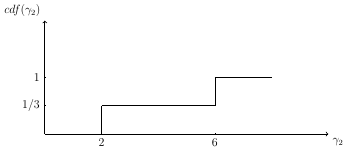
\includegraphics[scale=0.7]{images/cdf2}
    \end{displaymath}


     \begin{displaymath}
       $$cdf(\gamma_{SC}) = \left\{ \begin{array}{ll}
          \frac{\gamma}{21} & 2 < \gamma_{SC} \leq 6 \\
          \frac{\gamma}{7} & 6 < \gamma_{SC} < 7 \\
          1 & \gamma_{SC} > 7
       \end{array} \right. $$
       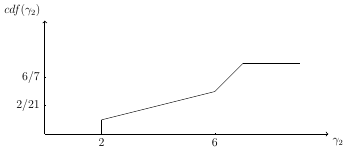
\includegraphics[scale=0.7]{images/cdfSC}
     \end{displaymath}

     Y como hemos dicho antes la \textit{pdf} por tanto vedndrá dada por: $pdf(\gamma_{SC}) = \frac{\partial (cdf_{SC}(\gamma_{SC}))}{\partial \gamma_{SC}}$, dando el siguiente resultado:

     \centering
     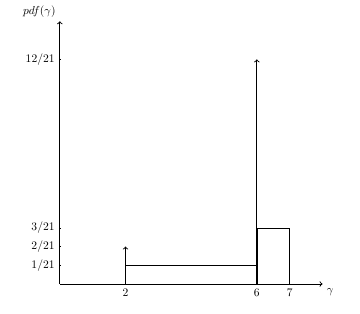
\includegraphics[scale=0.7]{images/18_SC.png}

     \newpage
     \item En MRC la $pdf_{MRC}$ o equivalente será la convolución de las pdfs de nuestros canales dando como resultado:
     \centering
     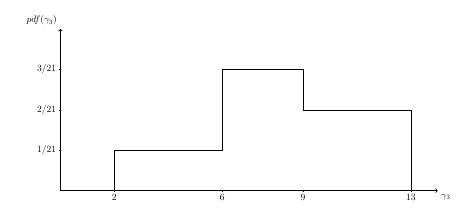
\includegraphics{images/18_2_2}

     $pdf(\gamma_{MRC}) =
     \begin{cases}
       \frac{1}{21} & 2 <  \gamma < 6 \\
       \frac{1}{7} & 6 <  \gamma < 9 \\
       \frac{2}{21} & 9 <  \gamma < 13 \\
       0 & resto
     \end{cases}$

     \raggedright
     \item En primer lugar obtenemos la eficiencia espectral multiplicando los bits de cada moduclación por $\frac{1}{2}$
     \begin{itemize}
       \centering
       \item BPSK : $R = 1 \cdot \frac{1}{2} = \frac{1}{2} $
       \item QPSK : $R = 2 \cdot \frac{1}{2} = 1 $
       \item 8PSK : $R = 3 \cdot \frac{1}{2} = \frac{3}{2} $
     \end{itemize}

    \raggedright
    Utilizando la fórmula proporcioanda por el enunciado obtenemos, la $\gamma_{min}$ , es decir la $\gamma$ necesaria para que la modulación funcione, dando así:
    \begin{itemize}
       \centering
      \item BPSK:   $\gamma_{min} \simeq$ 1.24
      \item QPSK:   $\gamma_{min} \simeq$  3
      \item 8PSK:   $\gamma_{min} \simeq$  5.48
    \end{itemize}

    \raggedright
    Teniendo en cuenta por tanto la pdf del primer canal, donde observamos que el valor máximo de este canal es 7, podemos por tanto decir que la modulación adaptativa de nuestro sistema será la siguiente:
    \begin{table}[htbp]
      \begin{center}
        \begin{tabular}{|l|l|}
          \hline
          NO TX & $0\leq\gamma<1.24$\\ \hline
          BPSK & $1.24\leq\gamma<3$ \\ \hline
          QPSK & $3\leq\gamma<5.48$ \\ \hline
          8PSK & $5.48\leq\gamma\leq7$ \\ \hline
        \end{tabular}
        \label{tabla:sencilla}
      \end{center}
    \end{table}

    \item Para hallar la tasa media transmitida, debemos hallar las probabilidades del funcionamiento de cada modulación:

    \begin{center}
      $P_{BPSK} = \int_{1.24}^{3}\frac{1}{7} \mathrm{d}x \approx 0.25$

      $P_{QPSK} = \int_{3}^{5.48}\frac{1}{7} \mathrm{d}x \approx 0.35$

      $P_{8PSK} = \int_{5.48}^{7}\frac{1}{7} \mathrm{d}x \approx 0.22$
    \end{center}

    Por tanto la tasa media de transmisión del sistema es:
    \begin{center}
      $\overline{R_b}$ = $B * g_c * b_{mod} * P_{mod}$ = $B*\frac{1}{2}*(1*0.25+2*0.35+3*0.22) = \boxed{\frac{B}{2}*1.61 = \overline{R_b}}$\
    \end{center}

    \item La calcularemos mediante la siguiente fórmula:

    \centering
    $\overline{BER} = P_{BPSK} * \overline{BER}_{BPSK} + P_{QPSK} * \overline{BER}_{QPSK} + P_{8PSK} * \overline{BER}_{8PSK}$

    \raggedright
    Las probabilidades de cada modulación fueron las calculadas en el apartado anterior.La $\overline{BER}$ de cada modulación se calculará mediante la siguiente fórmula:

    \centering
    $\overline{BER}_{REG} = \int_{\gamma_{ini}}^{\gamma_{fin}}BER_{REG}(\gamma)*pdf_{REG}(\gamma) \mathrm{d}\gamma$

    \raggedright
    La $BER_{REG}(\gamma)$ viene dado por el enunciado:   $0,2exp(-\gamma/(2R - 1))$. Y la $pdf_{REG}(\gamma)$ vendrá dada por la pdf de cada región que debe ser calculada de forma individual, esto quiere decir que entre cada rango de snr's para cada modulación el área debe ser 1.



    Aplicando lo anterior, la altura de cada pdf será:
    \begin{itemize}
    \item BPSK $\rightarrow \frac{1}{3-1.24} = \frac{1}{1.76}$
    \item QPSK $\rightarrow \frac{1}{5.48-3} = \frac{1}{2.48}$
    \item 8PSK $\rightarrow \frac{1}{7-5.48} = \frac{1}{1.52}$
    \end{itemize}

    Aplicamos para cada modulación la fórmula:

    $\overline{BER}_{BPSK} = \int_{1.24}^{3}0.2*e^{\frac{-\gamma}{2^{0.5-1}}}*\frac{1}{1.76} \mathrm{d}\gamma = 2.23*10^{-3}$

    $\overline{BER}_{QPSK} = \int_{3}^{5.48}0.2*e^{\frac{-\gamma}{2^{1-1}}}*\frac{1}{2.48} \mathrm{d}\gamma = 3.67*10^{-3}$

    $\overline{BER}_{8PSK} = \int_{5.48}^{7}0.2*e^{\frac{-\gamma}{2^{1.5-1}}}*\frac{1}{1.52} \mathrm{d}\gamma = 6.8*10^{-3}$

    Con los datos obtenidos sustituimos en la fórmula inicial:


    \centering
    $\overline{BER} =0.25 *  2.23*10^{-3} + 0.35 * 3.67*10^{-3} + 0.22 * 6.8*10^{-3} = \boxed{3.34*10^{-3}=\overline{BER}}$

    \raggedright
    \item Como no se aplica en este caso \textit{waterfilling}, suponemos que transmitimos 1 W todo el tiempo y por tanto $P_{TX} = 1 (\overline{P_{TX}} = 1)$ y potencia del ruido unitaria.

    La $\gamma$ recibida $\rightarrow$ $\gamma_{RX} = P_{TX} * \widetilde{\gamma}$, como $P_{TX}=1$ $\rightarrow$ $\gamma_{RX} =\widetilde{\gamma}$.

    La capacidad media ergódica viene dada por:
    \begin{center}
      $C_{ERG}(\widetilde{\gamma}) = B*\int_{0}^{\infty}log_2(1+\gamma_{RX}) * pdf(\gamma_{RX}) \mathrm{d}\gamma= B*(log_2(1+2)*\frac{1}{3}+log_2(1+2)*\frac{1}{3}) = 1.09*B$
    \end{center}

    Al ser una pdf con dos únicos valores, solo hay que tener en cuenta dichas probabilidades y que cada uno transmite 1W.


    \item Si implementamos \textit{waterfilling}, hay que tener en cuenta que la potencia transmitida será:
    \begin{center}
      $P_n = \lambda-\frac{1}{\gamma}_n$
   \end{center}

   Como ya hemmos establecido en el anterior apartado, la potencia media es 1 W, y por tanto:
   \begin{center}
     $\overline{P} = \frac{1}{3}*P_1+\frac{2}{3}*P_2$

     $1 = \frac{1}{3}*(\lambda-\frac{1}{2}) +  \frac{2}{3}*(\lambda-\frac{1}{6}) = \frac{\lambda}{3} - \frac{1}{6} +  \frac{2*\lambda}{6} - \frac{2}{18} = \boxed{\frac{23}{18}= \lambda}$
   \end{center}

   Teniendo $\lambda$, podemos hallar las potencias instantáneas:
   \begin{center}
     $P_1 = \frac{23}{18}-\frac{1}{2} = \boxed{\frac{14}{18} = P_1}$

     $P_2 = \frac{23}{18}-\frac{1}{6} = \boxed{\frac{20}{18} = P_2}$
   \end{center}

   Por tanto, la capacidad media ergódica es:
   \begin{center}
     $\overline{C}_{ERG} = B*[log_2(1+2*\frac{14}{18})*\frac{1}{3}+log_2(1+6*\frac{20}{18})*\frac{2}{3}] = \boxed{2.41*B = \overline{C}}$
   \end{center}

   \item Aplicando que la $P_{TX}$ sería inversamente proporcional a la $\gamma$ en el receptor (c: factor proporcionalidad), la potencia transmitida seguirá la pdf del MRC e integrando su pdf teniendo en cuenta que cada $P_{TX}$ es la inversa al valor del canal, obtendré la potencia media.(pdf del MRC calculado en apartado 2).

   \begin{center}
     $\overline{P}_{TX} = c *\int_{2}^{13}\frac{1}{\gamma_{MRC}}*pdf(\gamma_{MRC}) \mathrm{d}\gamma_{MRC}  = c*(\int_{2}^{6}\frac{1}{\gamma_{MRC}}*\frac{1}{21} \mathrm{d}\gamma_{MRC}+ \int_{6}^{9}\frac{1}{\gamma_{MRC}}*\frac{3}{21} \mathrm{d}\gamma_{MRC} +\int_{9}^{13}\frac{1}{\gamma_{MRC}}*\frac{2}{21} \mathrm{d}\gamma_{MRC}) = c * (\frac{1}{21}*[ln(\gamma_{MRC})]_2^6 +\frac{3}{21}*[ln(\gamma_{MRC})]_6^9+\frac{2}{21}*[ln(\gamma_{MRC})]_9^{13}) = \boxed {c*0.145 = \overline{P}_{TX}} $
   \end{center}

   \item En el caso de un canal AWGN con una pdf cuyo valor fuera una delta en 2, la diversidad del sistema es $\infty$. En nuestro sistema tenemos la pdf calculada en el apartado b), al ser mejor (puesto que ofrece mejores valores de SNR) tendríamos una ganancia \"mayor que infinito\", por tanto, la diversidad es $\infty$.
  \end{enumerate}

\end{document}
